\section{Results}
\label{sec:results}
All numbers are test results, in percent, as mean $\pm$ standard deviation over three seeds, unless stated.
The three seeds share the same writer-disjoint splits.

\subsection{RQ1: separating writers}
\Cref{tab:main} compares our model with the baselines.
On held-out writers the student reaches an EER of $2.35\pm0.12$ on IAM and $7.30\pm0.29$ on CVL (AUC 0.996 and 0.968).
Frozen DINOv2-small features, the teacher without any training on handwriting, give 5.44 and 15.02, so the student halves the error of the teacher on both corpora; HOG and an untrained CNN are far behind.
The 95\% bootstrap intervals over writers are wide (1.7 to 4.2 on IAM, 4.7 to 12.0 on CVL, per seed) because only 99 and 62 writers are available.
Test error is higher than validation error (IAM $0.90\pm0.31$, CVL $5.81\pm0.15$), which shows how optimistic the validation numbers were.
At a strict operating point the picture is weaker: with the false reject rate fixed at 1\%, the false accept rate is $10.1\pm1.2\%$ on IAM and $80.2\pm12.4\%$ on CVL, and at 10\% it is 0 and $3.5\pm0.4\%$.
The content-matched CVL pairs are therefore the hard case, and a single page pair is not enough evidence for a high-stakes decision.
On validation, an untrained encoder with batch-normalisation statistics adapted to the data already reaches 8.5\% on IAM and 21.3\% on CVL, which suggests that corpus-level cues such as scanner and paper carry part of the IAM signal.

\begin{table}[t]
\caption{Single-reference test results over all page pairs. The untrained CNN is averaged over three seeds; HOG and frozen DINOv2 have no training and are deterministic.}
\label{tab:main}
\centering\scriptsize
\setlength{\tabcolsep}{3pt}
\resizebox{\columnwidth}{!}{\begin{tabular}{lcccc}
\toprule
& \multicolumn{2}{c}{IAM} & \multicolumn{2}{c}{CVL} \\
Model & EER & AUC & EER & AUC \\
\midrule
Random CNN & 22.27$\pm$0.22 & 0.873$\pm$0.002 & 34.33$\pm$0.40 & 0.734$\pm$0.001 \\
HOG & 14.10 & 0.949 & 23.59 & 0.839 \\
DINOv2-small (frozen) & 5.03 & 0.992 & 16.00 & 0.911 \\
\midrule
Ours, 1 seed(s) & \textbf{0.48} & \textbf{1.000} & \textbf{5.90} & \textbf{0.984} \\
\bottomrule
\end{tabular}
}
\end{table}

\Cref{fig:train} shows validation EER and loss for the three seeds; after the best epoch the validation EER plateaus and fluctuates between about 3.5\% and 4.3\%, so the selected checkpoint is chosen from a noisy plateau.
The per-seed results (\Cref{tab:seeds}) differ by at most 0.3 EER on IAM and 0.7 on CVL, so the reported means are stable across seeds.

\begin{figure*}[t]
\centering
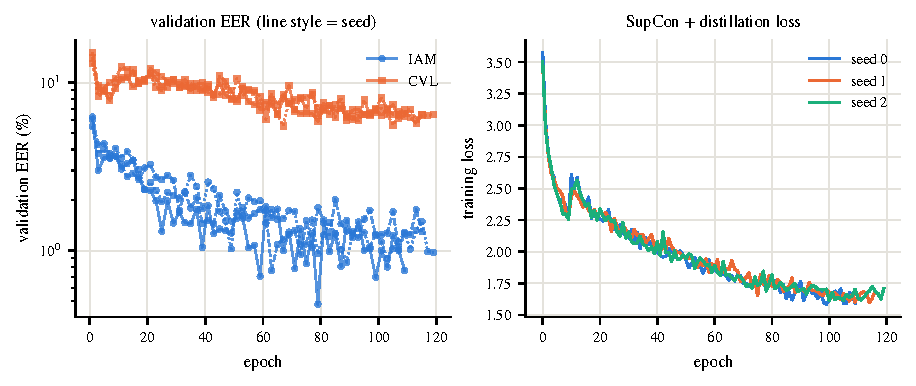
\includegraphics[width=\textwidth]{figures/fig_training_curves}
\caption{Validation EER (left, log scale; line style = seed) and training loss (right) of the three main runs.}
\label{fig:train}
\end{figure*}

\begin{table}[t]
\caption{Per-seed test results (EER, \%) and the share of inconclusive CVL verdicts.}
\label{tab:seeds}
\centering\scriptsize
\setlength{\tabcolsep}{2.5pt}
\resizebox{\columnwidth}{!}{\begin{tabular}{lccccc}
\toprule
Seed & IAM EER & CVL EER & Firemaker p4 & Firemaker p3 & CVL inconcl. (\%) \\
\midrule
0 & 2.20 & 7.16 & 3.00 & 31.40 & 7.8 \\
1 & 2.50 & 7.71 & 3.40 & 31.80 & 8.8 \\
2 & 2.36 & 7.04 & 3.60 & 32.80 & 8.9 \\
\bottomrule
\end{tabular}
}
\end{table}

\subsection{RQ2: more reference pages and fusion rules}
\Cref{fig:multiref} evaluates $N=1,2,3$ references on one fixed set of writers (45 on IAM, 62 on CVL, the writers with at least four pages), so that the writer set does not change with $N$.
With the centroid rule, the one used for calibration, EER falls from $2.25\pm0.05$ to $1.57\pm0.11$ and $1.22\pm0.12$ on IAM, and from $6.76\pm0.38$ to $5.22\pm0.54$ and $5.19\pm0.73$ on CVL.
On the 17 IAM writers with at least six pages, five references give $0.81\pm0.22$ against $1.96\pm0.31$ for one; CVL has too few such writers (three) for $N=5$.
The fusion rule matters.
On CVL the maximum of the cosine similarities is best at $N=3$ ($3.31\pm0.20$, against $5.99\pm0.71$ for the mean and $5.13\pm0.18$ for the two largest), while on IAM the centroid is best at three references and the maximum at two.
The centroid was fixed on validation, where it was best; that the maximum is better on test CVL is a post-hoc observation that we have not confirmed on separate data.
The seed-0 bootstrap intervals for $N=1$ and $N=3$ overlap (CVL centroid 3.6 to 10.8 and 2.3 to 9.0), so the gain from extra references is consistent in direction but not established for the population of writers.

\begin{figure*}[t]
\centering
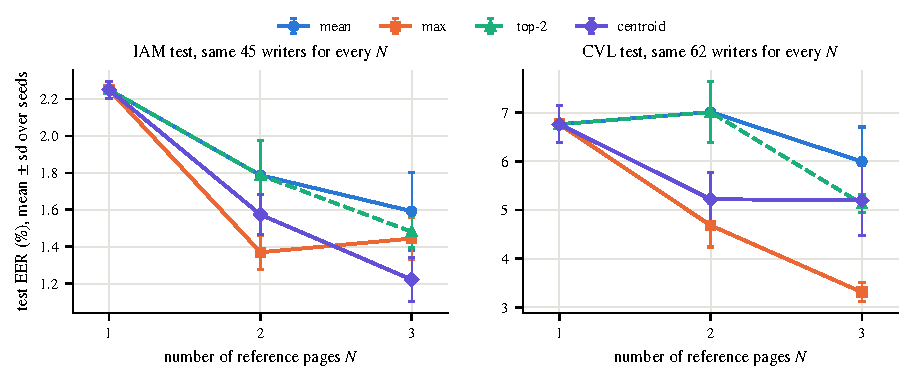
\includegraphics[width=\textwidth]{figures/fig_multiref_test}
\caption{Test EER against the number of reference pages for the four fusion rules, on one fixed set of writers for every $N$ (mean $\pm$ sd over three seeds). More references help, and the maximum rule is best on CVL.}
\label{fig:multiref}
\end{figure*}

\subsection{RQ3: cross-corpus transfer and disguise}
\Cref{tab:fm} and \Cref{fig:fm} use Firemaker, which differs in scanner and protocol and was never used for training, validation or thresholds.
For ordinary writing (page 1 against the self-written page 4) the EER is $3.33\pm0.25$ (AUC 0.994), close to IAM, so the representation transfers.
It does not survive a deliberate change of writing.
Upper-case copying raises the EER to $23.87\pm0.47$ and the disguised page to $32.00\pm0.59$.
The mean same-writer cosine falls from 0.978 to 0.906 and 0.874, while the mean other-writer cosine stays at about 0.79: disguise moves genuine pairs towards impostors.
A writer who simply changes style can therefore be rejected by the system, and the same effect would help a forger who copies a style.

\begin{table}[t]
\caption{Firemaker (250 writers): page 1 against pages 4, 2 and 3 of the same writers.}
\label{tab:fm}
\centering\scriptsize
\setlength{\tabcolsep}{2.5pt}
\resizebox{\columnwidth}{!}{\begin{tabular}{lcccc}
\toprule
Pair (same writer) & EER & AUC & Same-writer cos. & Other-writer cos. \\
\midrule
p1 vs p4 (natural, self-written) & 3.33$\pm$0.25 & 0.994$\pm$0.000 & 0.978$\pm$0.004 & 0.790$\pm$0.031 \\
p1 vs p2 (upper case) & 23.87$\pm$0.47 & 0.847$\pm$0.005 & 0.906$\pm$0.013 & 0.791$\pm$0.029 \\
p1 vs p3 (disguised) & 32.00$\pm$0.59 & 0.747$\pm$0.012 & 0.874$\pm$0.017 & 0.791$\pm$0.030 \\
\bottomrule
\end{tabular}
}
\end{table}

\begin{figure}[t]
\centering
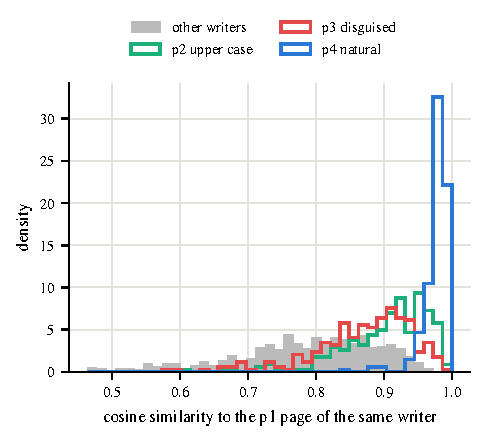
\includegraphics[width=\columnwidth]{figures/fig_firemaker}
\caption{Cosine similarity to the page 1 of the same writer on Firemaker (seed 0). Natural writing is clearly separated from other writers; disguise and upper case overlap them.}
\label{fig:fm}
\end{figure}

\subsection{RQ4: training ingredients}
\Cref{tab:abl} lists validation EER for six variants against the full model, all trained for 40 epochs with one seed.
No ingredient shows a clear benefit.
Removing distillation (4.38 against 5.35 mean EER), content-matched batches (4.57) or augmentation (4.88) gives a lower error than the full model, and mean pooling, no mining and eight patches (5.29, 5.25, 5.15) are within 0.2 of it.
The seed-to-seed spread of the main runs is about 0.2 in mean validation EER (3.19, 3.57 and 3.31), so only differences above that deserve attention, and with one seed per variant we cannot tell whether the lower values of the three variants are real.
What we can say is that, in this short schedule, none of the five training ingredients is demonstrated to help; the 120-epoch main model (mean validation EER 3.19 to 3.57) is better than every 40-epoch variant, which suggests that training length matters more than any single ingredient, although the two schedules also differ in warm-up and patience.

\begin{table}[t]
\caption{Ablations on validation (EER, \%; 40 epochs, one seed). The 120-epoch main model reaches a mean of 3.19 to 3.57 over three seeds.}
\label{tab:abl}
\centering\scriptsize
\setlength{\tabcolsep}{3pt}
\resizebox{\columnwidth}{!}{\begin{tabular}{lccc}
\toprule
Variant & IAM EER & CVL EER & Mean \\
\midrule
Full model (40 epochs) & 1.72 & 8.98 & 5.35 \\
No distillation & 1.22 & 7.53 & 4.38 \\
Mean pooling & 2.47 & 8.10 & 5.29 \\
No content-matched batches & 1.71 & 7.42 & 4.57 \\
No writer mining & 2.05 & 8.45 & 5.25 \\
8 patches per page & 2.53 & 7.77 & 5.15 \\
No augmentation & 1.74 & 8.02 & 4.88 \\
\bottomrule
\end{tabular}
}
\end{table}

\subsection{Calibrated verdicts}
Raw cosine scores are not probabilities: their expected calibration error is 0.22 on both corpora.
Platt scaling reduces it to 0.070 and 0.076, and isotonic regression to 0.009 and 0.020, all fitted on validation only.
\Cref{tab:verdict} gives the three-way verdict for three references.
On CVL, 8.5\% of trials are inconclusive; of the 91.5\% that are decided, 2.8\% are wrong.
IAM is separable on validation, so the 99th percentile of impostor scores lies below the 1st percentile of genuine scores; we then use one threshold and no inconclusive band (error 0.7\%), and the IAM verdict should not be read as evidence that the problem is easy (\Cref{sec:discussion}).

\begin{table}[t]
\caption{Three-way verdict on test trials with three references (centroid rule), thresholds from validation only.}
\label{tab:verdict}
\centering\scriptsize
\setlength{\tabcolsep}{2.5pt}
\resizebox{\columnwidth}{!}{\begin{tabular}{lccccc}
\toprule
Corpus & Consistent & Likely forged & Inconclusive & Error (decided) & ECE (Platt) \\
\midrule
IAM & 49.7$\pm$0.2 & 50.3$\pm$0.2 & 0.0$\pm$0.0 & 0.68$\pm$0.13 & 0.070$\pm$0.006 \\
CVL & 47.8$\pm$0.8 & 43.7$\pm$1.3 & 8.5$\pm$0.5 & 2.82$\pm$0.21 & 0.076$\pm$0.011 \\
\bottomrule
\end{tabular}
}
\end{table}

\begin{figure}[t]
\centering
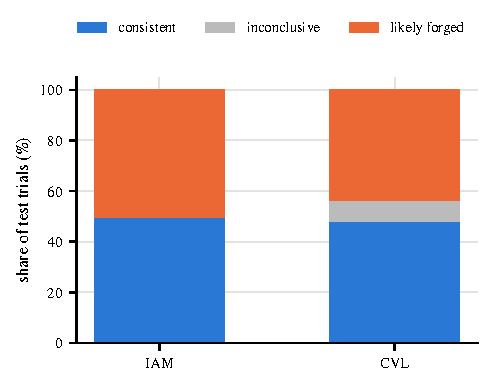
\includegraphics[width=\columnwidth]{figures/fig_verdict}
\caption{Share of test trials judged consistent, inconclusive and likely forged (mean over three seeds, three references).}
\label{fig:verdict}
\end{figure}

\begin{figure*}[t]
\centering
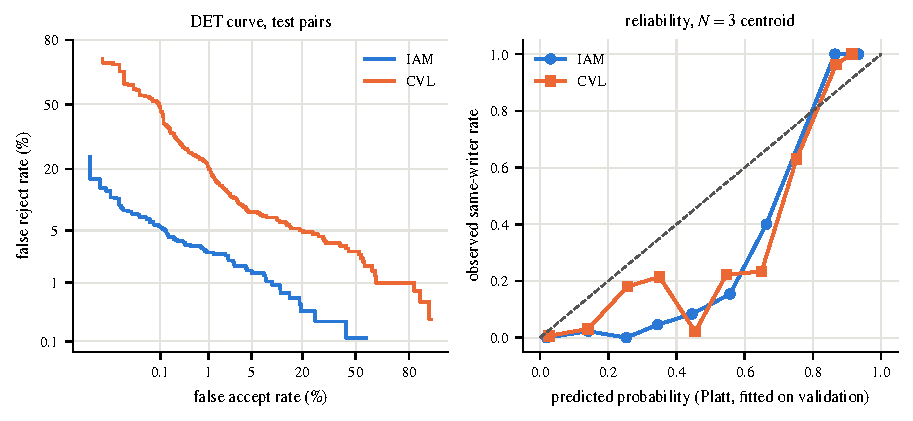
\includegraphics[width=\textwidth]{figures/fig_det_calibration}
\caption{Left: DET curves on test page pairs. Right: reliability of the Platt-calibrated probability for three references (calibrator fitted on validation); the Platt sigmoid is over-confident in the middle range (for example, predicted 0.66 against observed 0.40 on IAM) and under-confident at the top, which is why isotonic regression has the lower ECE.}
\label{fig:det}
\end{figure*}

\subsection{Synthetic pages}
\Cref{tab:syn} tests the 1362 font-rendered pages of the Kaggle set (and 990 real pages by unknown writers as a control) against every real test page, using the validation threshold at the 99th percentile of impostor scores.
Font renderings are accepted for 0.03\% of page pairs on IAM and for none on CVL, but unrelated real pages are accepted at a similar rate, and all score far below same-writer pairs.
Per page, 5.0\% of font pages (IAM threshold) are accepted by at least one of the 99 test writers, against 17.2\% of the real control pages.
The test therefore shows that fonts are not mistaken for real writers in this scan domain; it says nothing about learned imitation.

\begin{table}[t]
\caption{Kaggle pages scored against real test pages (single reference, validation threshold).}
\label{tab:syn}
\centering\scriptsize
\setlength{\tabcolsep}{2.5pt}
\resizebox{\columnwidth}{!}{\begin{tabular}{llccc}
\toprule
Corpus & Kaggle pages & Pairs accepted (\%) & Mean cosine & Pages accepted by $\geq$1 writer (\%) \\
\midrule
IAM & font-rendered & 0.033$\pm$0.023 & 0.47$\pm$0.01 & 5.0$\pm$2.3 \\
IAM & real, unknown writer & 0.144$\pm$0.035 & 0.52$\pm$0.00 & 17.2$\pm$4.9 \\
CVL & font-rendered & 0.000$\pm$0.000 & 0.39$\pm$0.02 & 0.0$\pm$0.0 \\
CVL & real, unknown writer & 0.003$\pm$0.003 & 0.48$\pm$0.02 & 0.4$\pm$0.2 \\
\bottomrule
\end{tabular}
}
\end{table}

\subsection{Where the model looks}
\Cref{fig:att} shows attention maps for four validation pages.
Removing the 25\% most attended patches lowers the cosine to a same-writer reference by 0.0043 on average, against 0.0022 for random patches (60 validation pairs, pair-to-pair standard deviation about 0.04).
The difference is too small to call the maps an explanation, so we use them only as a description of where the pooling puts weight.

\begin{figure*}[t]
\centering
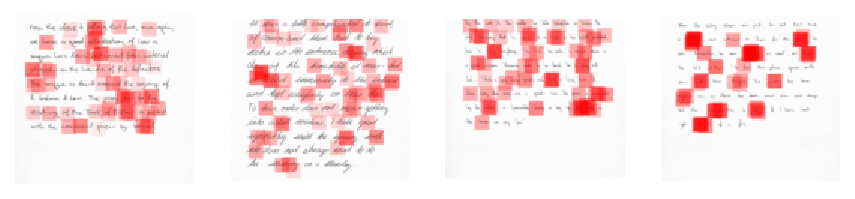
\includegraphics[width=\textwidth]{figures/fig_attention}
\caption{Attention weights (red, opacity proportional to weight) on four IAM validation pages.}
\label{fig:att}
\end{figure*}
